\chapter{Clustering-based Matrix Factorization for Leoline Shopping Prediction}
\label{chp:cbmf}
\section{Limitation of TRIMF}
In Chapter \ref{chp:trimf}, we introduced TRIMF. It's a matrix tri-factorization method for cross-domain recommendation. However, it has some limitations which restricts its scalability and extensibility.

First, when data are coming from multiple sources(e.g click, pageview, add cart), TRIMF treats every source equally and put each of them into a matrix which is very sparse. When solving the object function, more matrix will increase the time complexity and space complexity. If we try to update $S$, every matrix is included so it will be very time-consuming.

What's more, in reality we can't ignore users with fewer actions. Thus the matrix will be much more sparse than the ones in our experiment, so we can't guarantee to acheive equal performance.

To solve these problems, we developed a framework based on clustering and scoring scheme (CBMF, Figure \ref{fig:cbmf}). CBMF firstly cluster users according to their behavior and demographic features, then automatically convert different types of actions into one matrix call action matrix, finally a matrix factorization method is applied in the action matrix. For users with enough actions, personalized recommendation is provided. Otherwise we provide a recommendation based on his/her cluster.

\begin{figure}

%\begin{Large}

\begin{center}
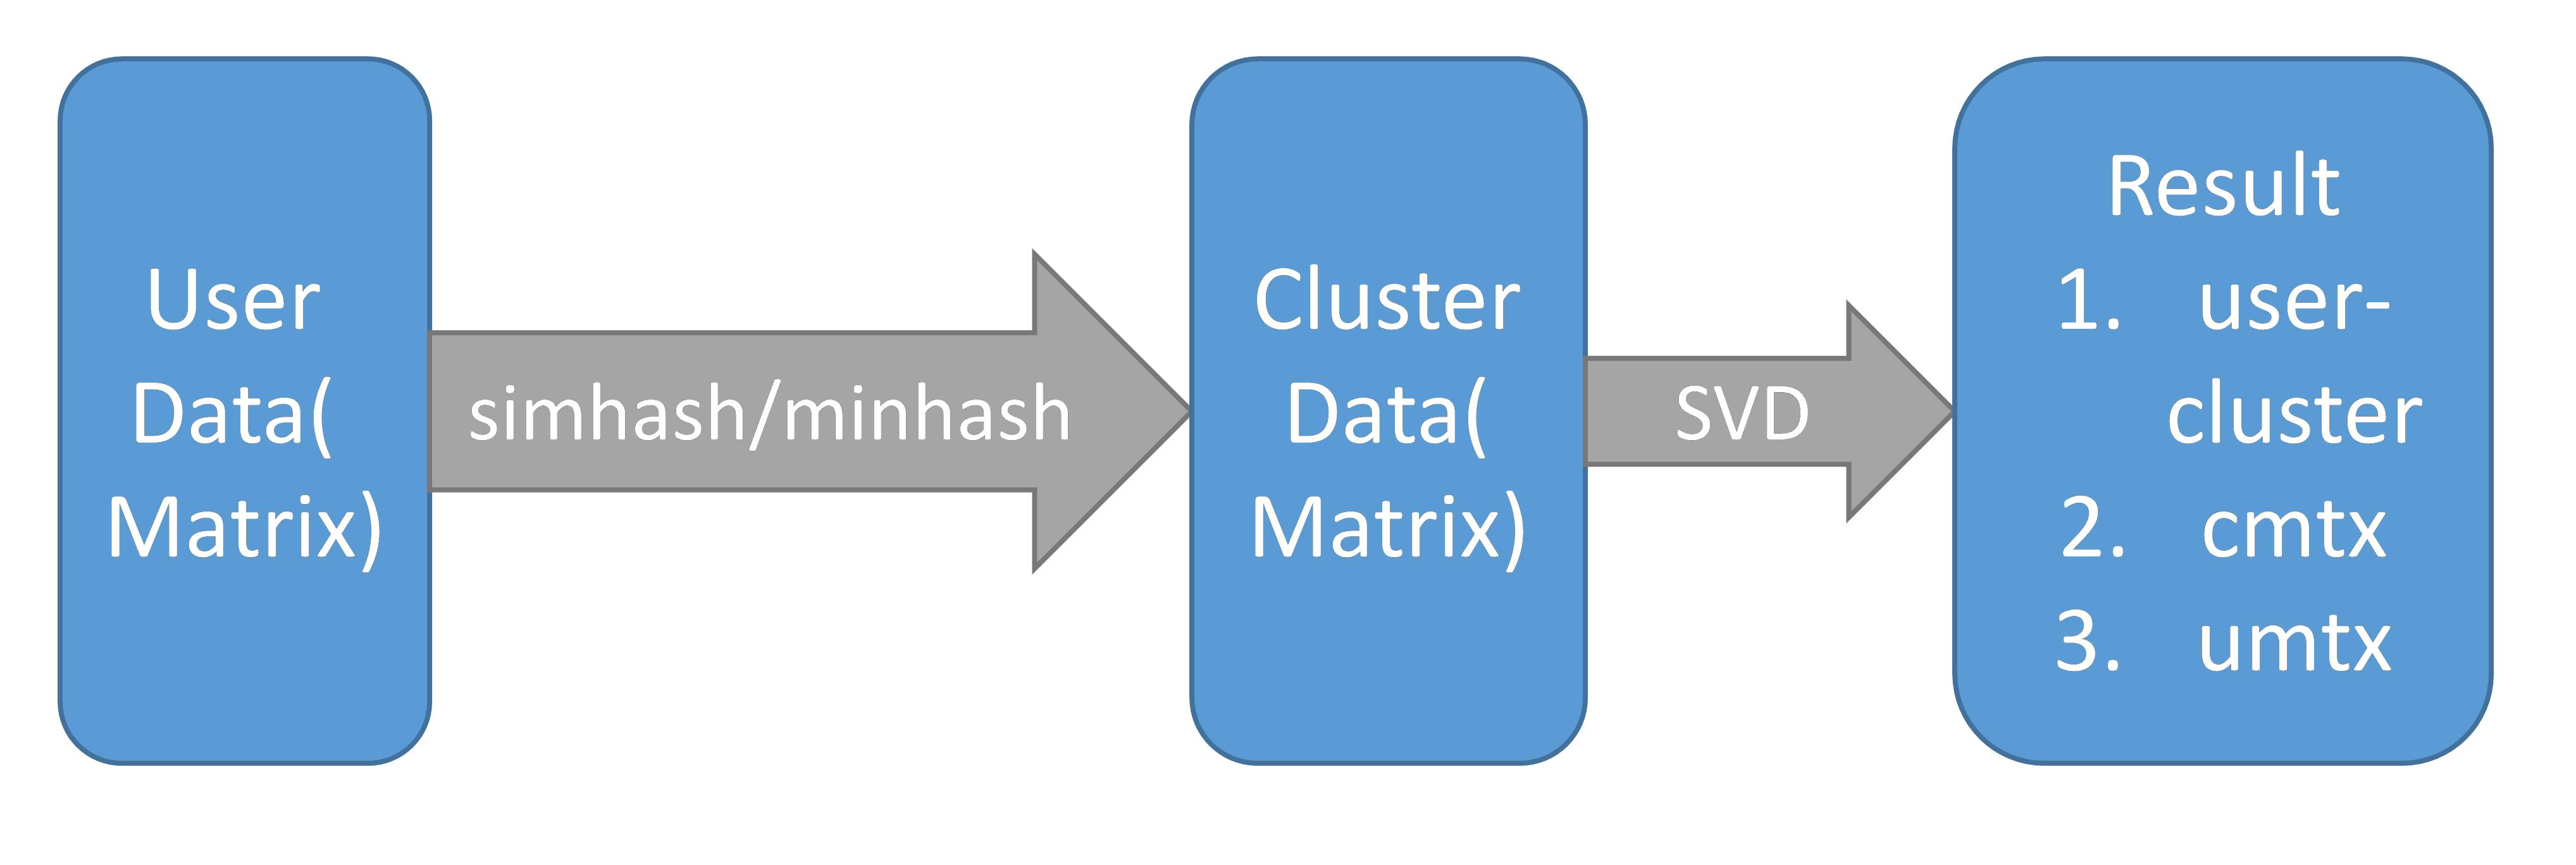
\includegraphics[width=400px]{fig/d} 
\caption{Framework of CBMF.}
\label{fig:cbmf}
\end{center}
\end{figure}





\section{Clustering method in CBMF}

Usually users' actions are unique and sparse, it'll be time-consuming if we want to cluster users using raw data. In Tencent, we have 800,000,000 users in total, and their feature vector size can be as large as 1,000,000. So if we want to speed up the phase, we must first convert large sparse user vector into a low dimension dense vector.

\subsection{Simhash}

Simhash is a kind of locality sensitive hashing(LSH). LSH is a hashing method that if we got two points $A,B$ which are close in their original space, after hashing we got $A',B'$, then $A',B'$ is still close in the new space. Thus we keep the relationship of distance among two spaces. 

The input of Simhash per user is $(feature_1, weight_1),..(feature_n,weight_n)$. The procedure of Simhash is in Algorithm \ref{algorithm:simhash}.

\begin{algorithm}[tb]
\caption{Simhash Algorithm for one instance.}
\begin{algorithmic}

\STATE {\bfseries Input:} $\X_U$, $h$\\
$\X_{U}$ : $(feature_1, weight_1),..(feature_n,weight_n)$ \\
$h$: a smooth hash function with $k$ bits after hashing\\

\STATE {\bfseries Initialize:} $r$(result vector) : $[0,0,0..0] \in \{0,1\}^k$

\FOR{ $i$ = 1 to $n$}

\STATE calculate $h(feature_i)$

\STATE $r = r + weight_i * h(feature_i)$

\ENDFOR

\FOR{ $i$ = 1 to $k$}
\IF {$r_i > 0$}
\STATE {$r_i = 1$}
\ELSE 
\STATE {$r_i = 0$}
\ENDIF
\ENDFOR

\STATE {\bfseries Output:} $r$

\end{algorithmic}
\label{algorithm:simhash}
\end{algorithm}

Assume that Simhash convert a vector $x$ into a 32-dimension binary vector $x'$. Actually $i_{th}$ bit of $x'$ is the sign of inner product of $x$ and $H_i = [h^1_i, h^2_i,...h^n_i]$, $H_i$ can be regarded as a hyperplane in original space. If two vector $x, y$ are in the same direction of $H_i$, then $x', y'$ is equal on $i_{th}$ bit. Thus we can use hamming distance in the low dimension to represent their similarity in original space.

\subsection{Minhash}

The similarity between two users $u_i , u_j$ is defined as the overlap between their item sets. $S(u_i, u_j) = \frac{C_{u_i} \cup C_{u_j}}{C_{u_i} \cap C_{u_j}}$, also known as the Jaccard coefficient. But doing this in real-time is clearly not scalable. However, we can achieve a provably sublinear time near-neighbor search technique by applying minhash.

MinHash is a probabilistic clustering method that assigns a pair of users to the same cluster with probability proportional to the overlap between the set of items that these users have voted for (clicked-on). In CBMF, minhashing is applied after simhashing, so every user has 32 items(bits). 

The basic idea in the Min-Hashing scheme is to randomly permute the set of items (S) and for each user $u_i$ compute its hash value $h(u_i)$ as the index of the first item under the permutation that belongs to the user’s item set $C_{u_i}$. And it's easy to show that the probability that two users will have the same hash function is exactly equal to their similarity or Jaccard coefficient.

Similar to \cite{Indyk:1998:ANN:276698.276876}, we can always concatenate $p$ hash-keys for
users, where $p \ge 1$, so the probability that any two users $u_i , u_j$ will agree on the concatenated hash-key is equal to $S(u_i , u_j )^p$. $p$ can be a parameter to control the number of clusters. If $p$ is large, then the clusters will be more refined thus the number of cluster will increase.

\subsection{Simhash \& Minhash using MapReduce}

MapReduce is a very simple model of computation over large clusters of machines that can handle processing of large amounts of data in relatively short periods of time and scales well with the number of machines. Our method Simhash and Minhash can be easily implemented using hadoop.

\subsubsection{Map phase}
In the map phase, we read the input records independently, in parallel, on different machines and map each input to a set of zero or more key-
value pairs. In our case, hadoop streaming is applied and each input instance is a user's vector(in sparse representation).

We first iterate the user's vector $u_i$, using Simhash to convert the vector to a 32-bit binary vector, the hashing function used in Simhash is FNV-32. Then Minhash is applied for $p$ times per user. We concatenate the $p$ Minhash values $Mnhs_i$ to obtain the cluster id of the user. Finally, the output is ( $Mnhs_i$, $u_i$), key is $Mnhs_i$, value is $u_i$. For users with enough actions, we output another pairs ( $user-id$, $u_i$). 

\subsubsection{Reduce phase}

In the reduce phase, our input has two form: ($Mnhs_i$, $u_i$) represents cluster-id and uservector. ($user-id$, $u_i$) represents an experienced user and its vector.
\begin{itemize}
\item For the cluster case: we obtain for each cluster-id the list of user-ids that belong to this cluster and prune away clusters with members less than 10. For each cluster-id, a joint vector is needed to represents all users in it. Thus we simply add scores from users to the joint vector, then we do a normalization to make the range of the vector between 0 and 1. The output has two parts: 
\begin{itemize}
\item user and the cluster he belongs to (userid, clusterid). 
\item cluster-id and its vector (cluster-id, cluster-vector).
\end{itemize}
\item For the user case: we simply output the normalized vector.

\end{itemize}

After the reduce phase, we have three tables(matrix). 1, user and his cluster-id. 2, cluster-id and its vector. 3, user and his vector.

\section{Feature construction in CBMF}

After clustering, we have many clusters and their corresponding actions, including click, purchase, pageview on different(overlap) items.

The naive way to handle those actions is to create a matrix $X_i$ for each action $i$. In matrix $X_i$, a row represents a cluster while a column represents an item, $X_{mn}$ represents the frequency of action that users in cluster $m$ had on item $n$. But simply creating such matrix may lead to data sparsity problems. Especially in the matrix standing for purchasing actions, even though we had already clustered similar users together. The data is still very sparse($0.01\%$) which may constrain our model from providing reasonable recommendation.

In CBMF, a scoring scheme is applied for each kind of action to put every action into a single matrix with proper score.For a specific item, a user may have four kinds of actions(click, purchase, pageview and uninterested). The idea behind the construction is that for a specific goal(e.g predict future purchase), what score should be given to an action depends on how much impact the action can have. 

For example, if we want to improve conversion rate, let $U_n$ denote the users who bought item $n$, $U$ denote the entire user set. Then the average conversion rate for a given item $n$ can be approximated by $Cvr(n_{all}) \approx \frac{|U_n|}{|U|}$. 
For a given action(e.g click), let $U_n^{click}$ denote the users who clicked item $n$. Then the conversion rate for users who had clicked this items can be approximated by $Cvr(n_{click}) \approx \frac{|U_n \cap U_n^{click}|}{|U_n^{click}|}$we compare the conversion rate of users who had this action with average, their log ratio $log(\frac{Cvr(n_{click})}{Cvr(n_{all})})$ is our initial score.

For each action with an item we calculate a score, in CBMF we used weighted scores and add them together. That is, for cluster $m$ and item $n$, if we have four scores:$s_1, s_2, s_3, s_4$ and their corresponding weights:$w_1, w_2, w_3, w_4$. We have $X_{mn} = \frac{\sum_{i=1}^4 w_i*s_i}{\sum_{i=1}^4 w_i}$. $w_i$ is the percentage of users who have this action compared to all users.

\section{Matrix factorization in CBMF}

Once the matrix are generated, we use Singular Value Decomposition(SVD) from mahout \footnote{https://mahout.apache.org/users/dim-reduction/dimensional-reduction.html}. The number of eigenvalues is set to 20 according to online test.

After SVD, we can provide recommendations to every user, for experienced users direct results are provides, otherwise we find his cluster-id and provide results for this cluster as our recommendation. We output our results to a online key-value dataset called TDE. Once a user comes, we search his id is TDE, the return value is our recommendation.

\section{Experiments and results analysis}

Our algorithm has gone online for about one months from 2014-04-01 to 2014-05-01 with $10\%~20\%$ users, in the chatting scenerio. That is, when you are chatting using QQ, an ad full of items will pop out in front of you. Most of the users will close it immediately, so $90\%$ of the users are new. And we need to provide results for every user, about 80,000,000.

After some days of parameter selection, CBMF's performance becomes stable since 2014-04-10.

There are three evaluation metrics: 
\begin{itemize}
\item [1] click-through-rate(CTR). 
\item [2] order amount per impression(OAPI)
\item [3] pay amount per impression(PAPI).
\end{itemize}

An impression is a measure of the number of times an ad is seen. The difference between OAPI and PAPI is that a user may place an order but didn't pay for it(he can cancel at any time).

\subsection{Baselines}

There are some others algorithms competing with CBMF, we split users into different disjoint sets. Each algorithm impact a set of users, and an ID is given to every algorithms, the ID of CBMF is 4312. The detail of other algorithms is shown below:

\begin{itemize}
\item 4312: CBMF, updates per hour.
\item 4313: Locally popular algorithm. Each user belongs to a cluster according to their age and gender, then the most popular items in this cluster are recommended. Real time algorithm.
\item 4314: Logistic regression algorithm, the feature consists users' demographic data, items' category data and their conjunctions. The algorithm updates per hour.
\item 4315: Globally popular algorithm. For every user, items with most-clicked are provided. Real time algorithm.
\item cpsf: Redirecting based algorithm, if a user had some positive(click, pageview, purchase) actions before, recommend popular items in the same category. If the user is new, recommend the most-clicked items in different category(avoid recommending items all from one category). Real time algorithm.

\end{itemize} 

\subsection{Click through rate}


\begin{figure}
\begin{center}
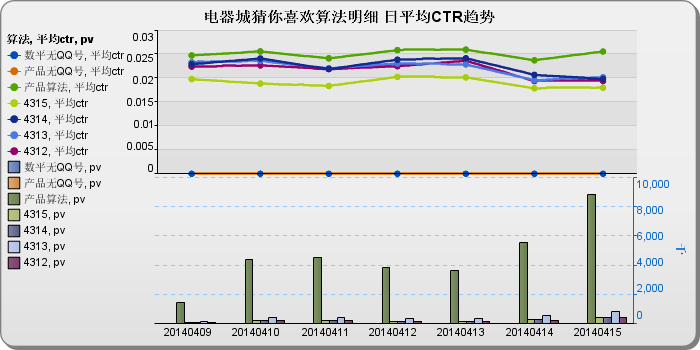
\includegraphics[width=400px]{fig/yixunexp/ctr0415.png}
\caption{\label{fig:ctr0415} CTR of online algorithms from 0409 to 0415.}

\end{center}
\end{figure}

\begin{figure}
\begin{center}

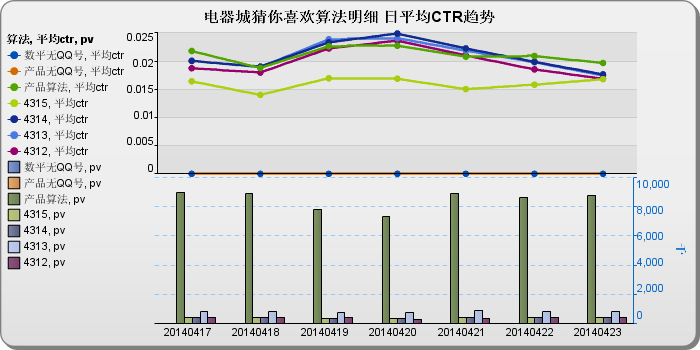
\includegraphics[width=400px]{fig/yixunexp/ctr0424.png}
\caption{\label{fig:ctr0424} CTR of online algorithms from 0417 to 0424.}
\end{center}
\end{figure}

In Figure \ref{fig:ctr0415} and Figure \ref{fig:ctr0424}, CTR of different online algorithms are shown. The id of CBMF is $4312$, the purple line. It can be seen that CBMF didn't rank first in CTR, but rather among the mid levels. This is because CBMF didn't optimize for CTR, it is designed for improving purchase rate. But because there is some similarity between click and purchase, so CBMF's CTR performance could not be too bad.

For other algorithms, we can see personalized algorithms perform better than global algorithm. 4315 has the lowest CTR because it just provide same recommendations to every user. Redirecting seems to work very well in CTR, since users may like to click items they are familiar with. Especially in our scenerio, the users are chatting while a panel full of viewed item poped out, he/she may not close it immediately. Instead, he/she may just review the items they clicked before.

\subsection{Order amount per impression}

\begin{figure}
\begin{center}

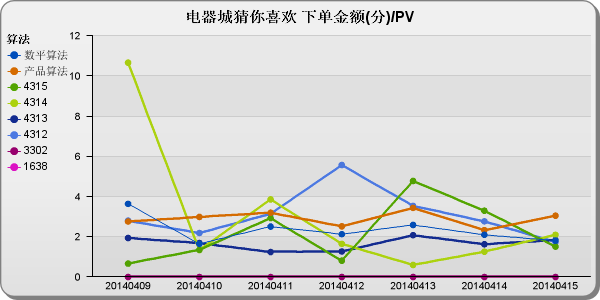
\includegraphics[width=400px]{fig/yixunexp/OAPI0415.png}
\caption{\label{fig:oapi0415} OAPI of online algorithms  from 0409 to 0415.}
\end{center}
\end{figure}

\begin{figure}
\begin{center}



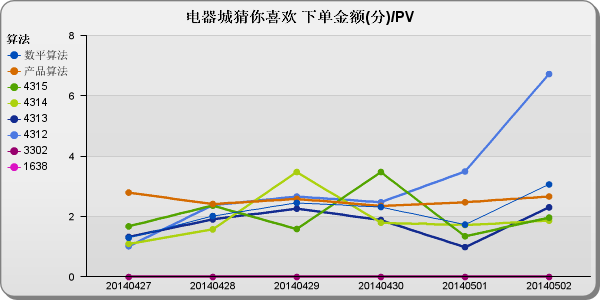
\includegraphics[width=400px]{fig/yixunexp/OAPI0427.png}
\caption{\label{fig:oapi0427} OAPI of online algorithms  from 0427 to 0502.}
\end{center}
\end{figure}

\begin{figure}
\begin{center}



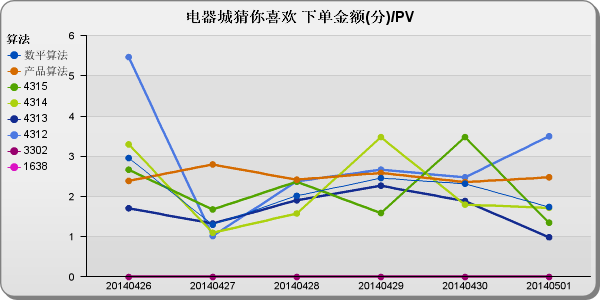
\includegraphics[width=400px]{fig/yixunexp/cvr0502.png}
\caption{\label{fig:oapi0426} OAPI of online algorithms  from 0426 to 0501.}
\end{center}
\end{figure}

\begin{table}[h]

%\begin{Large}

\begin{center}
\begin{tabular}{| c | c | c | c |}
\hline
Algorithm ID & Average OAPI in Figure \ref{fig:ctr0415} & Average OAPI in Figure \ref{fig:ctr0424} & Average total OAPI \\
\hline
4315 &2.21 & 2.87 & 2.64\\
\hline
4314 &\textbf{3.33} & 2.65& 2.86\\
\hline
4312 &3.25& \textbf{3.97}& \textbf{3.65}\\
\hline
4313 & 1.93 & 2.31& 2.12\\
\hline
cpsf & 3.04& 2.98 & 3.01\\
\hline
\end{tabular}
\caption{\label{tbl:cvravg} Average OAPI of online algorithms.}
\end{center}
%\end{Large}
\end{table}

In Figure \ref{fig:oapi0415} and Figure \ref{fig:oapi0427}, OAPI of different online algorithms are shown. The id of CBMF is $4312$, the blue line. In Figure \ref{fig:oapi0415}, we can see that CBMF is relatively stable and its performance are among the best. In Figure \ref{fig:oapi0427} , CBMF outperforms other algorithms significantly. In Table \ref{tbl:cvravg}, we can see that although CBMF may not be the best in one week's performance due to insufficient data. But its overall OAPI is the highest.

If we look at the Figure carefully we can find that, CBMF tends to achieve better performance in holidays( 4-11, 4-12, 5-1, 5-2 are all Chinese holidays). This may because in holidays, users tends to buy something which they are long for while in ordinary days users may buy some necessary first. CBMF captures users' desire to buy something they like instead of they need, so CBMF will achieve better performance in holidays.


\subsection{Pay amount per impression}

\begin{figure}
\begin{center}

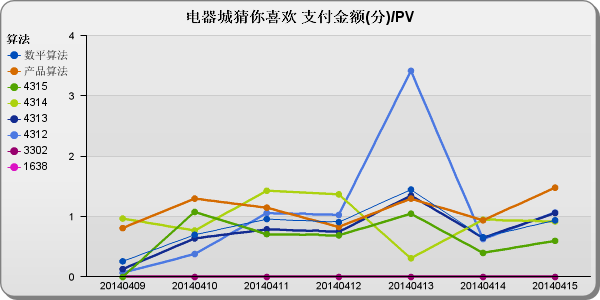
\includegraphics[width=400px]{fig/yixunexp/PAPI0415.png}
\caption{\label{fig:papi0415} PAPI of online algorithms  from 0409 to 0415.}
\end{center}
\end{figure}

\begin{figure}
\begin{center}

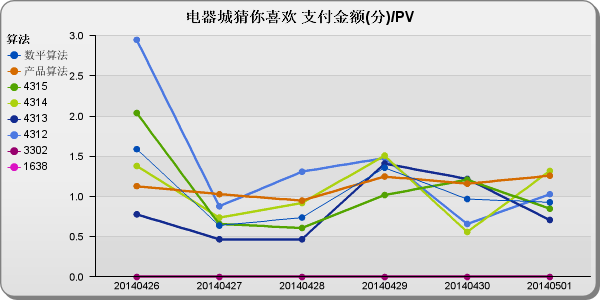
\includegraphics[width=400px]{fig/yixunexp/PAPI0421.png}
\caption{\label{fig:papi0501} PAPI of online algorithms  from 0426 to 0501.}
\end{center}
\end{figure}

In Figure \ref{fig:papi0415} and Figure \ref{fig:papi0501}, OAPI of different online algorithms are shown. The id of CBMF is $4312$, the blue line. We can see that CBMF outperforms other algorithms in these two periods. Different from the observations in OAPI, users may have high OAPI in Mondays and Sundays, that may because users may not pay right after they place their order. After thinking carefully, they may finally pay which leads to the delay effect in OAPI.

\subsection*{Overall evaluation}
From the three evluation metrics, we can see CBMF can acheive better conversion rate, moderate click through rate comparing to others. 



